% ------------------------------------------------------------------------------
% TYPO3 Version 10.0 - What's New (French Version)
%
% @author	Michael Schams <schams.net>
% @translator	Paul Blondiaux
% @reviewer	Pierrick Caillon
% @license	Creative Commons BY-NC-SA 3.0
% @link		http://typo3.org/download/release-notes/whats-new/
% @language	French
% ------------------------------------------------------------------------------

\section{Changements pour les développeurs}
\begin{frame}[fragile]
	\frametitle{Changements pour les développeurs}

	\begin{center}\huge{Chapitre 4~:}\end{center}
	\begin{center}\huge{\color{typo3darkgrey}\textbf{Changements pour les développeurs}}\end{center}

\end{frame}

% ------------------------------------------------------------------------------
% TYPO3 Version 10.0 - Breaking Changes

\begin{frame}[fragile]
	\frametitle{Changements pour les développeurs}
	\framesubtitle{Changements cassants}

	\small
		À l'attention des développeurs~: Certaines classes PHP, interfaces, alias de classes,
		propriétés, méthodes, constantes, options et variables globales, etc. furent marquées
		dépréciées en TYPO3 v9.

		\vspace{0.2cm}

		En accord avec la \textbf{politique de dépréciation} de TYPO3, ces composants ont été
		retirés dans TYPO3 v10.0.

		\vspace{0.2cm}

		Sont inclus certains hooks, annotations PHP (comme \texttt{@inject} et
		\texttt{@validate}), et aussi des portées changées (par exemple de
		«~\texttt{public}~» à «~\texttt{protected}~»).

		\vspace{0.2cm}

		Activez le journal de dépréciation, testez soigneusement votre code et lisez
		les journaux pour identifier tout problème potentiel. Utilisez l'
		\href{https://docs.typo3.org/m/typo3/reference-coreapi/master/en-us/ApiOverview/ExtensionScanner/Index.html}{analyseur d'extension (en)}
		intégré pour obtenir un rapport complet des incompatibilités des extensions.

	\normalsize

\end{frame}

% ------------------------------------------------------------------------------
% Feature | 88643 | New Mail API based on symfony/mailer and symfony/mime
% Breaking | 88643 | Removed Swiftmailerswiftmailer Dependency

\begin{frame}[fragile]
	\frametitle{Changements pour les développeurs}
	\framesubtitle{Nouvelle API Mail}

	\begin{itemize}
		\item SwiftMailer est remplacé par des bibliothèques plus modernes~: 

			\begin{itemize}
				\item \texttt{symfony/mime} pour la création de messages
				\item \texttt{symfony/mailer} pour l'envoi de mails
			\end{itemize}

		\item La fonction PHP \texttt{mail()} n'est plus supportée.

			\begin{itemize}\smaller
				\item[\ding{228}] Il est recommandé de passer sur \texttt{sendmail} ou \texttt{smtp}.
			\end{itemize}\normalsize

		\item Les plugins ou les transports pour SwiftMailer personnalisés nécessiteront une migration.

		\item Voir la \href{https://symfony.com/doc/current/mailer.html}{documentation de Symfony (en)}
			pour plus d'informations sur l'utilisation des capacités de la nouvelle API Mail.
	\end{itemize}

\end{frame}

% ------------------------------------------------------------------------------
% Feature | 84112 | Symfony dependency injection for core and Extbase

\begin{frame}[fragile]
	\frametitle{Changements pour les développeurs}
	\framesubtitle{Injection et gestion de dépendances Symfony (1)}

	\begin{itemize}
		\item Le paquet \texttt{symfony/dependency-injection} est intégré et utilisé pour gérer
			les dépendances à travers le système et l'injection de dépendances pour les classes.

		\item Cette approche vise à remplacer l'injection de dépendances d'Extbase

		\item Ainsi, les classes doivent être ajustées et il faut éviter (lorsque possible)~:

			\begin{itemize}\small
				\item \texttt{\textbackslash
					TYPO3\textbackslash
					CMS\textbackslash
					Extbase\textbackslash
					Object\textbackslash
					ObjectManager}
				\item \texttt{\textbackslash
					TYPO3\textbackslash
					CMS\textbackslash
					Core\textbackslash
					Utility\textbackslash
					GeneralUtility::makeInstance()}
			\end{itemize}\normalsize

	\end{itemize}

\end{frame}

% ------------------------------------------------------------------------------
% Feature | 84112 | Symfony dependency injection for core and Extbase

\begin{frame}[fragile]
	\frametitle{Changements pour les développeurs}
	\framesubtitle{Injection et gestion de dépendances Symfony (2)}

	% decrease font size for code listing
	\lstset{basicstyle=\tiny\ttfamily}

	\begin{itemize}
		\item Les options de configuration incluent~:

			\begin{itemize}
				\item L'association automatique «~autowiring~» (voir l'exemple ci-dessous)
				\item L'association manuelle
					(voir \href{https://docs.typo3.org/c/typo3/cms-core/master/en-us/Changelog/10.0/Feature-84112-SymfonyDependencyInjectionForCoreAndExtbase.html}{journal des changements (en)})
				\item Fonctionnalités avancées
					(voir \href{https://docs.typo3.org/c/typo3/cms-core/master/en-us/Changelog/10.0/Feature-84112-SymfonyDependencyInjectionForCoreAndExtbase.html}{journal des changements (en)})
			\end{itemize}

		% \smaller For example "autowiring":\normalsize

\begin{lstlisting}
# Configuration/Services.yaml
services:
  _defaults:
    autowire: true
    autoconfigure: true
    public: false

  Your\Namespace\:
    resource: '../Classes/*'
\end{lstlisting}

		\item Voir la \href{https://symfony.com/doc/current/service_container.html}{documentation de Symfony (en)} pour plus d'informations.

	\end{itemize}

\end{frame}

% ------------------------------------------------------------------------------
% Feature | 88769 | Introduce a generic EventDispatcher based on PSR-14
% Feature | 88770 | Add PSR-14 EventDispatcher logic based on DI

\begin{frame}[fragile]
	\frametitle{Changements pour les développeurs}
	\framesubtitle{Gestionnaire d'événements (1)}

	\begin{itemize}
		\item Un nouveau système «~EventDispatcher~» est ajouté pour remplacer les Hooks et
			les concepts de Signal/Slot.

		\item Ce système est basé sur la \href{https://www.php-fig.org/psr/psr-14}{norme PSR-14 (en)}
			permettant aux développeurs d'injecter des comportement dans l'application de façon
			simple et systématique.

		\item PSR-14 contient quatre composants~:

			\begin{itemize}
				\item Un objet \textbf{EventDispatcher} permettant de déclencher un événement.
				\item Un objet \textbf{ListenerProvider} contenant les écouteurs enregistrés pour
					tous les événements.
				\item Un ou plusieurs objets \textbf{Event} qui sont appelés depuis le cœur de TYPO3
					ou les extensions («~Émetteurs~»)
				\item Un ou plusieurs objets \textbf{Listeners} (habituellement dans les extensions
					ou les paquets PHP) qui sont enregistrés.
			\end{itemize}

% Short-Term goal is to deprecate SignalSlot dispatcher in TYPO3 v10,
% and migrate all signals to the EventDispatcher.

	\end{itemize}

\end{frame}

% ------------------------------------------------------------------------------
% Feature | 88769 | Introduce a generic EventDispatcher based on PSR-14
% Feature | 88770 | Add PSR-14 EventDispatcher logic based on DI

\begin{frame}[fragile]
	\frametitle{Changements pour les développeurs}
	\framesubtitle{Gestionnaire d'événements (2)}

	% decrease font size for code listing
	\lstset{basicstyle=\tiny\ttfamily}

	Exemple d'implémentation

	\begin{itemize}\smaller
		\item[\ding{202}] Ajoutez la balise \texttt{event.listener} au fichier \texttt{Configuration/Services.yaml}~:

\begin{lstlisting}
services:
  Vendor\Example\EventListener\NullMailer:
    tags:
      - { name: event.listener, identifier: 'myListener', event: TYPO3\CMS\Core\Mail\Event\AfterMailerInitializationEvent, before: 'redirects, anotherIdentifier' }
\end{lstlisting}

		\item[\ding{203}] Implémentez votre objet événement~:

\begin{lstlisting}
namespace Vendor\Example\EventListener;

class NullMailer
{
  public function __invoke(AfterMailerInitializationEvent $event): void
  {
    $event->getMailer()->injectMailSettings(['transport' => 'null']);
  }
}
\end{lstlisting}

	\end{itemize}\normalsize

\end{frame}

% ------------------------------------------------------------------------------
% Feature | 88769 | Introduce a generic EventDispatcher based on PSR-14
% Feature | 88770 | Add PSR-14 EventDispatcher logic based on DI

\begin{frame}[fragile]
	\frametitle{Changements pour les développeurs}
	\framesubtitle{Gestionnaire d'événements (3)}

	% decrease font size for code listing
	\lstset{basicstyle=\tiny\ttfamily}

	\begin{itemize}
		\item La liste des écouteurs d'événements (\textit{Event Listeners}) est disponible en Backend~:\newline
			\smaller
				(l'extension \texttt{EXT:lowlevel} est nécessaire)
			\normalsize
	\end{itemize}

	\begin{figure}
		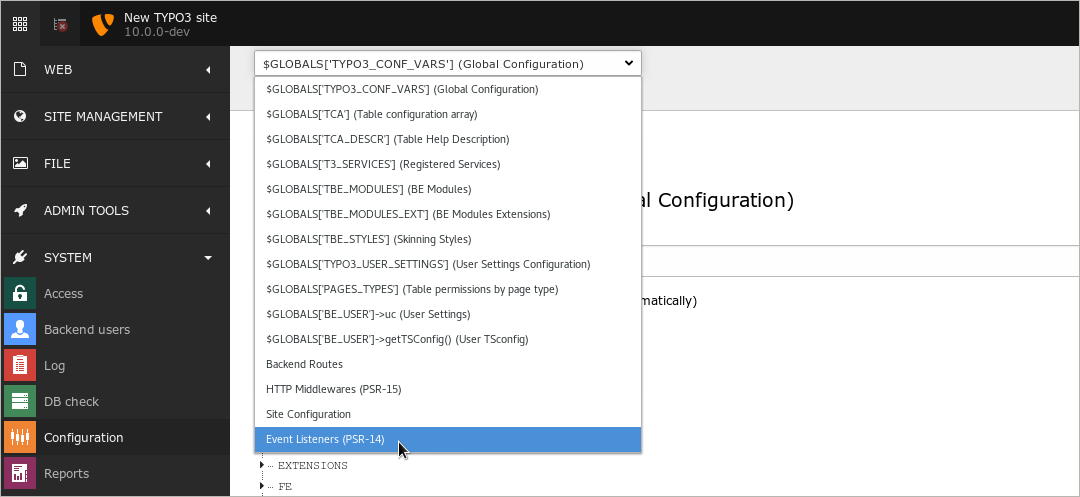
\includegraphics[width=0.70\linewidth]{ChangesForDevelopers/88770-PSR14-EventDispatcher.png}
	\end{figure}

\end{frame}


% ------------------------------------------------------------------------------
% Feature | 88769 | Introduce a generic EventDispatcher based on PSR-14
% Feature | 88770 | Add PSR-14 EventDispatcher logic based on DI

\begin{frame}[fragile]
	\frametitle{Changements pour les développeurs}
	\framesubtitle{Gestionnaire d'événements (4)}

	% decrease font size for code listing
	\lstset{basicstyle=\tiny\ttfamily}

	\begin{itemize}
		\item Bonnes pratiques~:

			\begin{itemize}
				\item N'implémentez qu'un seul écouteur par classe PHP et utilisez \texttt{\_\_invoke()}
					comme nom de méthode.
				\item Ajouter le suffixe «~\texttt{Event}~» au nom des classes PHP d'événement
					lors de leur création.
				\item Placez la classe événement dans un dossier approprié, i.e. \texttt{Classes/Database/Event}.
				\item Utilisez la forme constructeur de l'injection de dépendances pour recevoir
					l'objet EventDispatcher si possible.
			\end{itemize}

		\item Remarque supplémentaire~:\newline
			\small
				Les événement fournit par le cœur TYPO3 respectent la politique de dépréciation,
				sauf pour le constructeur dont les arguments peuvent changer.
			\normalsize

	\end{itemize}

\end{frame}

% ------------------------------------------------------------------------------
% Feature | 88799 | Use PSR-3 interface for logging

\begin{frame}[fragile]
	\frametitle{Changements pour les développeurs}
	\framesubtitle{Interface de journalisation PSR-3}

	\begin{itemize}
		\item Le framework de journalisation de TYPO3 (en particulier LogLevel et LogManager)
			implémente l'\href{https://www.php-fig.org/psr/psr-3/}{interface de journalisation PSR-3 (en)}.

		\item PSR-3 est une méthode standardisée permettant aux bibliothèques de recevoir un objet
			\texttt{Psr\textbackslash
				Log\textbackslash
				LoggerInterface} et d'écrire des journaux de façon simple et universelle.

			\item Ceci permet aux développeurs d'utiliser des journaliseurs personnalisés et d'interagir
				avec d'autres systèmes de journalisation.

	\end{itemize}

\end{frame}

% ------------------------------------------------------------------------------
% Breaking | 88182 | jsfunc.inline.js has been dropped
% Breaking | 88427 | jsfunc.evalfield.js has been removed
% Breaking | 88667 | Removed additionalJavaScriptSubmit from FormEngine
% Deprecation | 88433 | Deprecate top.openUrlInWindow

\begin{frame}[fragile]
	\frametitle{Changements pour les développeurs}
	\framesubtitle{Options et fonctions JavaScript (1)}

	\begin{itemize}
		\item Les fichiers JavaScript suivants ont été retirés~:

			\begin{itemize}
				\item \texttt{jsfunc.inline.js}
				\item \texttt{jsfunc.evalfield.js}
			\end{itemize}

			\begin{itemize}\smaller
				\item[\ding{228}] Utilisez plutôt \texttt{TYPO3/CMS/Backend/FormEngineValidation}.
			\end{itemize}\normalsize

		\item Des gestionnaires de soumission additionnels pouvaient être ajoutés avec l'option
			\texttt{additionalJavaScriptSubmit}. Elle est retirée.

			\begin{itemize}\smaller
				\item[\ding{228}] À la place, créez et inscrivez un module AMD.
			\end{itemize}\normalsize

		\item La fonction JavaScript globale \texttt{top.openUrlInWindow()} est marquée dépréciée.

	\end{itemize}

\end{frame}

% ------------------------------------------------------------------------------
% Breaking | 88411 | TBE_EDITOR.typo3form removed
% Deprecation | 88432 | Replaced md5js with an AMD module
% Deprecation | 88428 | top.rawurlencode and top.str_replace
% Deprecation | 88651 | Replace TYPO3/CMS/Backend/SplitButtons with TYPO3/CMS/Backend/DocumentSaveActions

\begin{frame}[fragile]
	\frametitle{Changements pour les développeurs}
	\framesubtitle{Options et fonctions JavaScript (2)}

	\begin{itemize}

		\item L'objet global \texttt{TBE\_EDITOR.typo3form} ainsi que \texttt{typo3FormFieldSet}
			et \texttt{typo3FormFieldGet} sont retirés.

		\item Le fichier \texttt{md5.js} est marqué déprécié.

			\begin{itemize}\smaller
				\item[\ding{228}] À la place, chargez le module AMD \texttt{TYPO3/CMS/Backend/Hashing/Md5} via RequireJS.
			\end{itemize}\normalsize

		\item Les fonctions globales JavaScript suivantes sont marquées dépréciées~:

		\begin{itemize}
			\item \texttt{top.rawurlencode()}
			\item \texttt{top.str\_replace()}
		\end{itemize}

		\item Le module \texttt{TYPO3/CMS/Backend.SplitButtons} est déprécié.

			\begin{itemize}\smaller
				\item[\ding{228}] Utilisez plutôt \texttt{TYPO3/CMS/Backend/DocumentSaveActions}.
			\end{itemize}\normalsize

 	\end{itemize}

\end{frame}

% ------------------------------------------------------------------------------
% Important | 87894 | Removed PHP Dependency algo26-matthiasidna-convert

\begin{frame}[fragile]
	\frametitle{Changements pour les développeurs}
	\framesubtitle{Domaines en UTF-8}

	\begin{itemize}
		\item PHP possède des fonctions natives de conversion d'un domaine de l'UTF-8 en forme IDNA ASCII
			(«~punicode~»), par exemple \href{https://www.php.net/manual/en/function.idn-to-ascii.php}{idn\_to\_ascii()}.

		\item Elles s'utilisent directement lorsque l'extension PHP
			«~\href{https://www.php.net/manual/en/book.intl.php}{intl}~» est installée.

		\item Si l'extension PHP n'est pas installée, le paquet \texttt{symfony/polyfill-intl-idn}
			fournit ces fonctions.

		\item Le paquet \texttt{algo26-matthias/idna-convert} qui était utilisé auparavant est retiré.

	\end{itemize}

\end{frame}

% ------------------------------------------------------------------------------
% Feature | 87665 | Introduce BitSet class

\begin{frame}[fragile]
	\frametitle{Changements pour les développeurs}
	\framesubtitle{Classe BitSet}

	% decrease font size for code listing
	\lstset{basicstyle=\tiny\ttfamily}

	\begin{itemize}
		\item Une classe pour gérer efficacement les indicateurs booléens est introduite~:\newline
			\texttt{TYPO3\textbackslash
				CMS\textbackslash
				Core\textbackslash
				Type\textbackslash
				BitSet}

		\item Par exemple~:

\begin{lstlisting}
define('PERMISSIONS_NONE', 0b0); // 0
define('PERMISSIONS_PAGE_SHOW', 0b1); // 1
define('PERMISSIONS_PAGE_EDIT', 0b10); // 2
define('PERMISSIONS_PAGE_DELETE', 0b100); // 4
define('PERMISSIONS_PAGE_NEW', 0b1000); // 8
define('PERMISSIONS_CONTENT_EDIT', 0b10000); // 16
define('PERMISSIONS_ALL', 0b11111); // 31

$bitSet = new \TYPO3\CMS\Core\Type\BitSet(PERMISSIONS_PAGE_SHOW | PERMISSIONS_PAGE_NEW);
$bitSet->get(PERMISSIONS_PAGE_SHOW); // true
$bitSet->get(PERMISSIONS_CONTENT_EDIT); // false
\end{lstlisting}

	\end{itemize}

\end{frame}

% ------------------------------------------------------------------------------
% Important | 87516 | Remove Core HTTP Request Handler Interface

\begin{frame}[fragile]
	\frametitle{Changements pour les développeurs}
	\framesubtitle{Gestionnaire de requêtes (1)}

	\begin{itemize}
		\item L'interface interne suivante est retirée en faveur du gestionnaire de requête PSR-15
			et des middlewares~:\newline
			\texttt{TYPO3\textbackslash
				CMS\textbackslash
				Core\textbackslash
				Http\textbackslash
				RequestHandlerInterface}

	\end{itemize}

\end{frame}

% ------------------------------------------------------------------------------
% Breaking | 88687 | Configure extbase request handlers via PHP

\begin{frame}[fragile]
	\frametitle{Changements pour les développeurs}
	\framesubtitle{Gestionnaire de requêtes (2)}

	% decrease font size for code listing
	\lstset{basicstyle=\tiny\ttfamily}

	\begin{itemize}
		\item La configuration du gestionnaire de requêtes Extbase ne s'effectue plus en TypoScript.

		\smaller\textbf{Ancienne} méthode par TypoScript~:\normalsize
\begin{lstlisting}
config.tx_extbase {
  mvc {
    requestHandlers {
      Vendor\Example\Mvc\Web\FrontendRequestHandler = Vendor\Example\Mvc\Web\FrontendRequestHandler
    }
  }
}
\end{lstlisting}

		\smaller\textbf{Nouvelle} Méthode par le fichier \texttt{Configuration/Extbase/RequestHandlers.php}~:\normalsize
\begin{lstlisting}
<?php
declare(strict_types = 1);

return [
  \Vendor\Example\Mvc\Web\FrontendRequestHandler::class,
];
\end{lstlisting}

	\end{itemize}

\end{frame}


% ------------------------------------------------------------------------------
% Deprecation | 88366 | Default caching framework cache names changed

\begin{frame}[fragile]
	\frametitle{Changements pour les développeurs}
	\framesubtitle{Framework de cache}

	% decrease font size for code listing
	\lstset{basicstyle=\tiny\ttfamily}

	\begin{itemize}
		\item Les caches suivants sont renommés~:

			\begin{itemize}\smaller
				\item \texttt{cache\_core} \textrightarrow\hspace{0.1cm}\texttt{core}
				\item \texttt{cache\_hash} \textrightarrow\hspace{0.1cm}\texttt{hash}
				\item \texttt{cache\_pages} \textrightarrow\hspace{0.1cm}\texttt{pages}
				\item \texttt{cache\_pagesection} \textrightarrow\hspace{0.1cm}\texttt{pagesection}
				\item \texttt{cache\_runtime} \textrightarrow\hspace{0.1cm}\texttt{runtime}
				\item \texttt{cache\_rootline} \textrightarrow\hspace{0.1cm}\texttt{rootline}
				\item \texttt{cache\_imagesizes} \textrightarrow\hspace{0.1cm}\texttt{imagesizes}
			\end{itemize}\normalsize

		\item Nouvelle méthode d'accès aux caches~:

\begin{lstlisting}
AVANT~:
$cacheManager->getCache('cache_core').

MAINTENANT~:
$cacheManager->getCache('core')
\end{lstlisting}

		\item Le préfixe \texttt{cf\_} est retiré des tables de base de données.
	\end{itemize}

\end{frame}

% ------------------------------------------------------------------------------
% Deprecation | 87550 | Use controller classes when registering plugins/modules

\begin{frame}[fragile]
	\frametitle{Changements pour les développeurs}
	\framesubtitle{Extbase et Fluid (1)}

	% decrease font size for code listing
	\lstset{basicstyle=\tiny\ttfamily}

	\begin{itemize}
		\item L'inscription des plugins/modules nécessite les noms qualifiés des classes~:

			\begin{itemize}\smaller
				\item \texttt{\textbackslash
					TYPO3\textbackslash
					CMS\textbackslash
					Extbase\textbackslash
					Utility\textbackslash
					ExtensionUtility::configurePlugin()}
				\item \texttt{\textbackslash
					TYPO3\textbackslash
					CMS\textbackslash
					Extbase\textbackslash
					Utility\textbackslash
					ExtensionUtility::registerModule()}
			\end{itemize}\normalsize

		\item Aussi, ne plus spécifier le nom de fournisseur avec le nom d'extension (premier argument).

			\begin{itemize}\smaller
				\item[\ding{228}] Utilisez «~\texttt{ExampleBlog}~» au lieu de «~\texttt{Vendor.ExampleBlog}~».
			\end{itemize}

		\item Exemple~:

\begin{lstlisting}
\TYPO3\CMS\Extbase\Utility\ExtensionUtility::configurePlugin(
  'ExampleBlog', // previously: 'Vendor.ExampleBlog'
  'pi1',
  [
    \Vendor\Example\Controller\BlogController::class => 'list,update,delete'
  ],
  [
    \Vendor\Example\Controller\BlogController::class => 'list,update,delete'
  ]
);
\end{lstlisting}

	\end{itemize}

\end{frame}

% ------------------------------------------------------------------------------
% Breaking | 87627 | Remove Property extensionName of AbstractController

\begin{frame}[fragile]
	\frametitle{Changements pour les développeurs}
	\framesubtitle{Extbase et Fluid (2)}

	\begin{itemize}
		\item La propriété \texttt{extensionName} de AbstractController est retirée.

			\begin{itemize}\smaller
				\item[\ding{228}] Utilisez alors \texttt{\textbackslash
					TYPO3\textbackslash
					CMS\textbackslash
					Extbase\textbackslash
					Mvc\textbackslash
					Request::getControllerExtensionName()}.
			\end{itemize}\normalsize

	\end{itemize}

\end{frame}

% ------------------------------------------------------------------------------
% Feature | 87457 | Use symfony/propertyinfo to gather doc block information

\begin{frame}[fragile]
	\frametitle{Changements pour les développeurs}
	\framesubtitle{Extbase et Fluid (3)}

	% decrease font size for code listing
	\lstset{basicstyle=\tiny\ttfamily}

	\begin{itemize}
		\item Les modèles Extbase supportent les noms de classe non qualifiés dans le bloc de documentation.

\begin{lstlisting}
use TYPO3\CMS\Extbase\Persistence\ObjectStorage;
use ExtbaseTeam\BlogExample\Domain\Model\Comment;

class Post
{
  /**
   * @var ObjectStorage<Comment>
   */
  public $comments;
}
\end{lstlisting}

	\end{itemize}

\end{frame}

% ------------------------------------------------------------------------------
% Breaking | 87957 | Validators are not registered automatically in Extbase anymore

\begin{frame}[fragile]
	\frametitle{Changements pour les développeurs}
	\framesubtitle{Extbase et Fluid (4)}

	% decrease font size for code listing
	\lstset{basicstyle=\tiny\ttfamily}

	\begin{itemize}
		\item Les validateurs ne sont plus inscrits automatiquement dans Extbase.
		\item Pour un modèle nommé
			\small\texttt{Vendor\textbackslash
				Example\textbackslash
				Domain\textbackslash
				Model\textbackslash
				Blog}\normalsize,\newline
			Extbase utilisait automatiquement le validateur
			\small\texttt{Vendor\textbackslash
				Example\textbackslash
				Domain\textbackslash
				Validator\textbackslash
				BlogValidator}\normalsize

		\item Les validateurs doivent être inscrits manuellement~:

\begin{lstlisting}
use Vendor\Example\Domain\Model\Blog;
use TYPO3\CMS\Extbase\Annotation as Extbase;
use TYPO3\CMS\Extbase\Mvc\Controller\ActionController;

class BlogController extends ActionController
{
  /**
   * @Extbase\Validate(param="blog", validator="Vendor\Example\Domain\Validator\BlogValidator")
   */
  public function showAction(Blog $blog)
  {
    // ...
  }
}
\end{lstlisting}

	\end{itemize}

\end{frame}

% ------------------------------------------------------------------------------
% Breaking | 87623 | Replace config.persistence.classes typoscript configuration (1)

\begin{frame}[fragile]
	\frametitle{Changements pour les développeurs}
	\framesubtitle{Extbase et Fluid (5) - Class Mapping (1)}

	% decrease font size for code listing
	\lstset{basicstyle=\tiny\ttfamily}

	\begin{itemize}
		\item La définition des associations entre champs et propriétés de la persistance en TypoScript
			n'est plus supportée~:

\begin{lstlisting}
config.tx_example_blog {
  persistence {
    classes {
      Vendor\Example\Domain\Model\Author {
        mapping {
          tableName = fe_users
          columns.name.mapOnProperty = fullname
        }
      }
    }
  }
}
\end{lstlisting}

	\end{itemize}

\end{frame}

% ------------------------------------------------------------------------------
% Breaking | 87623 | Replace config.persistence.classes typoscript configuration (2)

\begin{frame}[fragile]
	\frametitle{Changements pour les développeurs}
	\framesubtitle{Extbase et Fluid (6) - Class Mapping (2)}

	% decrease font size for code listing
	\lstset{basicstyle=\tiny\ttfamily}

	\begin{itemize}
		\item Les associations entre les modèles et la base doivent être indiquées dans le fichier
			\texttt{Configuration/Extbase/Persistence/Classes.php}~:

\begin{lstlisting}
<?php
declare(strict_types = 1);

return [
  \Vendor\Example\Domain\Model\Author::class => [
    'tableName' => 'fe_users',
    'properties' => [
      'fullname' => [
        'fieldName' => 'name'
      ]
    ]
  ]
];
\end{lstlisting}

		\begin{itemize}\smaller
			\item[\ding{228}] NB~: le nom de la propriété et le champ de base de données ont été interchangés~!\newline
				Avant~:\tabto{1.6cm}\texttt{<db-field>.mapOnProperty = <property>}\newline
				Maintenant~:\tabto{1.6cm}\texttt{properties.<property>.fieldname = <db-field>}
		\end{itemize}\normalsize

	\end{itemize}

\end{frame}

% ------------------------------------------------------------------------------
% Breaking | 87594 | Harden Extbase

\begin{frame}[fragile]
	\frametitle{Changements pour les développeurs}
	\framesubtitle{Extbase et Fluid (7)}

	% decrease font size for code listing
	\lstset{basicstyle=\smaller\ttfamily}

	\begin{itemize}
		\item Les fichiers de classe utilisent le mode «~types stricts~» et les indications de type scalaires.

\begin{lstlisting}
<?php
declare(strict_types=1);
\end{lstlisting}

		% Method signatures in Extbase classes have been updated.
		\item Ceci lève des erreurs PHP fatales lorsque les signatures de méthode dans les extensions
			ne sont pas compatibles avec l'interface ou la classe parente.

		\item Voir \href{https://forge.typo3.org/issues/87594}{forge \#87594 (en)}
			pour la liste complète des fichiers et leurs changements.

		\item Cette tâche est toujours en cours et de nouveaux changements seront effectués.

	\end{itemize}

\end{frame}

% ------------------------------------------------------------------------------
% Breaking | 87937 | TCA option selicon_field_path removed
% Breaking | 87989 | TCA option setToDefaultOnCopy removed
% Breaking | 87936 | TCA for sys_history removed

\begin{frame}[fragile]
	\frametitle{Changements pour les développeurs}
	\framesubtitle{Changements TCA}

	\begin{itemize}
		\item Les options TCA suivantes sont retirées~:

			\begin{itemize}
				\item \texttt{\$TCA[\$tableName]['ctrl']['selicon\_field\_path']}
				\item \texttt{\$TCA[\$tableName]['ctrl']['setToDefaultOnCopy']}
			\end{itemize}

			\begin{itemize}\smaller
				\item[\ding{228}] Lors de la copie d'enregistrements, il faut utiliser un DataHandler pour réinitialiser les champs.
			\end{itemize}\normalsize

		\item L'entièreté du TCA de \texttt{sys\_history} est retiré et le champ \texttt{pid} en base est abandonné.
			L'accès à \texttt{\$GLOBALS['TCA']['sys\_history']} déclenche un avertissement PHP.

	\end{itemize}

\end{frame}

% ------------------------------------------------------------------------------
% Breaking | 88527 | Overriding custom values in User Authentication derivatives

\begin{frame}[fragile]
	\frametitle{Changements pour les développeurs}
	\framesubtitle{Services et classes d'authentification utilisateur (1)}

	\begin{itemize}
		\item La classe abstraite suivante est restructurée~:\newline
			\small\texttt{TYPO3\textbackslash
				CMS\textbackslash
				Core\textbackslash
				Authentication\textbackslash
				AbstractUserAuthentication}\normalsize
		\item Ce qui impact ces deux sous-classes directes~:

			\begin{itemize}
				\item \texttt{BackendUserAuthentication}
				\item \texttt{FrontendUserAuthentication}
			\end{itemize}

		\item Et affecte les propriétés~:

			\begin{itemize}
				\item \texttt{sessionTimeout}
				\item \texttt{gc\_time}
				\item \texttt{sessionDataLifetime}
				\item \texttt{loginType}
			\end{itemize}

	\end{itemize}

\end{frame}

% ------------------------------------------------------------------------------
% Breaking | 88646 | Removed inheritance of AbstractService from AbstractAuthenticationService

\begin{frame}[fragile]
	\frametitle{Changements pour les développeurs}
	\framesubtitle{Services et classes d'authentification utilisateur (2)}

	\begin{itemize}

		\item Cette classe n'hérite plus de
			\smaller\texttt{AbstractService}~:\normalsize\hspace{0.1cm}
			
			\smaller\texttt{\textbackslash
				TYPO3\textbackslash
				CMS\textbackslash
				Core\textbackslash
				Authentication\textbackslash
				AbstractAuthenticationService}\normalsize

		\item Ce changement peut toucher certains hook et les fournisseurs d'authentification alternatifs.

		\item Il est conseillé aux développeurs de vérifier leurs services d'authentification et de les mettre
			à jour au besoin.

	\end{itemize}

\end{frame}

% ------------------------------------------------------------------------------
% Deprecation | 87882 | File related controllers moved to EXT:filelist

\begin{frame}[fragile]
	\frametitle{Changements pour les développeurs}
	\framesubtitle{Contrôleurs de Filelist}

	\begin{itemize}
		\item Les contrôleurs suivant sont déplacés dans \texttt{EXT:filelist}~:

			\begin{itemize}\small
				\item \texttt{CreateFolderController}
				\item \texttt{EditFileController}
				\item \texttt{FileUploadController}
				\item \texttt{RenameFileController}
				\item \texttt{ReplaceFileController}
			\end{itemize}\normalsize

		\item En conséquence, leur espace de nom est changé en\newline
			\texttt{\textbackslash
				TYPO3\textbackslash
				CMS\textbackslash
				Filelist\textbackslash
				Controller\textbackslash
				File}

		\vspace{0.2cm}

		\small
			Remarque~: Utilisez le FAL TYPO3 comme API et ajoutez vos fonctionnalités avec votre contrôleur
			au lieu de réutiliser les contrôleurs \textbf{internal} listés ci-dessus.
		\normalsize

	\end{itemize}

\end{frame}

% ------------------------------------------------------------------------------
% Deprecation | 88499 | BackendUtility::getViewDomain()

\begin{frame}[fragile]
	\frametitle{Changements pour les développeurs}
	\framesubtitle{URL de prévisualisation Frontend}

	% decrease font size for code listing
	\lstset{basicstyle=\tiny\ttfamily}

	\begin{itemize}
		\item La méthode statique suivante est marquée dépréciée~:\newline
			\smaller\texttt{\textbackslash
				TYPO3\textbackslash
				CMS\textbackslash
				Backend\textbackslash
				Utility\textbackslash
				BackendUtility::getViewDomain()}\normalsize

		\item Substituez la méthode par la détection du site à l'aide de l'identifiant de
			page dans le backend TYPO3.
		\item Par Exemple~:

\begin{lstlisting}
$pageId = 123;
$site = GeneralUtility::makeInstance(SiteFinder::class)->getSiteByPageId($pageId);
$url = $site->getRouter()->generateUri($pageId, ['type' => 13]);
\end{lstlisting}

	\end{itemize}

\end{frame}

% ------------------------------------------------------------------------------
% Deprecation | 88406 | setCacheHash/noCacheHash options in ViewHelpers and UriBuilder

\begin{frame}[fragile]
	\frametitle{Changements pour les développeurs}
	\framesubtitle{cHash dans l'UriBuilder et les ViewHelpers}

	% decrease font size for code listing
	\lstset{basicstyle=\smaller\ttfamily}

	\begin{itemize}
		\item Les deux méthodes d'UriBuilder suivantes sont dépréciées~:

			\begin{itemize}
				\item \texttt{UriBuilder->setUseCacheHash()}
				\item \texttt{UriBuilder->getUseCacheHash()}
			\end{itemize}

		\item Ce qui impact de nombreux ViewHelpers Fluid~:
	\end{itemize}
	\vspace{-0.4cm}
	\begin{columns}[T]
		\begin{column}{.05\textwidth}
		\end{column}
		\begin{column}{.45\textwidth}
			\begin{itemize}\smaller
				\item \texttt{f:form}
				\item \texttt{f:link.action}
				\item \texttt{f:link.page}
				\item \texttt{f:link.typolink}
				\item \texttt{f:uri.action}
			\end{itemize}\normalsize
		\end{column}
		\begin{column}{.45\textwidth}
			\begin{itemize}\smaller
				\item \texttt{f:uri.page}
				\item \texttt{f:uri.typolink}
				\item \texttt{f:widget.link}
				\item \texttt{f:widget.uri}
			\end{itemize}\normalsize
		\end{column}
	\end{columns}
	\vspace{0.2cm}
	\begin{itemize}
		\item ... comme l'option TypoScript «~\texttt{useCacheHash}~».
	\end{itemize}

\end{frame}

% ------------------------------------------------------------------------------
% Breaking | 88540 | Changed Request Workflow for Frontend Requests

\begin{frame}[fragile]
	\frametitle{Changements pour les développeurs}
	\framesubtitle{Traitement des requêtes Frontend (1)}

	% decrease font size for code listing
	\lstset{basicstyle=\smaller\ttfamily}

	\begin{itemize}
		\item Le traitement des requêtes Frontend est modifié.

		\item Les composants impliqués sont tous construits en utilisant les middlewares PSR-15,
			les gestionnaire de requêtes PSR-15, et le TypoScriptFrontendController (TSFE) global
			depuis TYPO3 v9.

		\item Ceci impacte le code lorsque le hook suivante et un session frontend sont utilisés~:\newline
			{\fontsize{7}{8}\selectfont\texttt{\$GLOBALS['TYPO3\_CONF\_VARS']['SC\_OPTIONS']['tslib/class.tslib\_fe.php']['hook\_eofe']}}

			\begin{itemize}\smaller
				\item[\ding{228}] Utilisez un middleware PSR-15 au lieu d'un hook,
					ou faites un appel explicite à \texttt{storeSessionData}
					dans le hook en PHP.
			\end{itemize}\normalsize

	\end{itemize}

\end{frame}

% ------------------------------------------------------------------------------
% Breaking | 88498 | Global data for TimeTracker statistics removed

\begin{frame}[fragile]
	\frametitle{Changements pour les développeurs}
	\framesubtitle{Traitement des requêtes Frontend (2)}

	% decrease font size for code listing
	\lstset{basicstyle=\smaller\ttfamily}

	\begin{itemize}
		\item Les valeurs globales suivantes sont retirées~:

			\begin{itemize}
				\item \texttt{\$GLOBALS['TYPO3\_MISC']['microtime\_start']}
				\item \texttt{\$GLOBALS['TYPO3\_MISC']['microtime\_end']}
				\item \texttt{\$GLOBALS['TYPO3\_MISC']['microtime\_BE\_USER\_start']}
				\item \texttt{\$GLOBALS['TYPO3\_MISC']['microtime\_BE\_USER\_end']}
			\end{itemize}

		\item À titre d'exemple, elles étaient utilisées par le cœur de TYPO3 dans le panneau d'administrateur
			et dans les en-têtes HTTP.

			\begin{itemize}\smaller
				\item[\ding{228}] Utilisez plutôt \texttt{TimeTracker->finish()}.
			\end{itemize}\normalsize

	\end{itemize}

\end{frame}


% ------------------------------------------------------------------------------
% Deprecation | 88569 | Locales::initialize() in favor of regular singleton instance
% Deprecation | 88473 | TypoScriptFrontendController->settingLocale

\begin{frame}[fragile]
	\frametitle{Changements pour les développeurs}
	\framesubtitle{Paramètres régionaux (1)}

	\begin{itemize}
		\item La méthode \texttt{Locales::initialize()} est marquée dépréciée.

			\begin{itemize}\smaller
				\item[\ding{228}] Utilisez plutôt \texttt{GeneralUtility::makeInstance(Locales::class)} ou une
				injection de dépendance pour récupérer une instance de la classe \texttt{Locales}.
			\end{itemize}\normalsize

		\item La fonctionnalité de la méthode suivante est marquée déprécié~:\newline
			\texttt{TypoScriptFrontendController->settingLocale()}.

			\begin{itemize}\smaller
				\item[\ding{228}] La fonction est disponible sous
				{\fontsize{8}{8}\selectfont\texttt{Locales::setSystemLocaleFromSiteLanguage()}.}
			\end{itemize}\normalsize

	\end{itemize}

\end{frame}

% ------------------------------------------------------------------------------
% Deprecation | 88559 | TSFE->sys_language_isocode

\begin{frame}[fragile]
	\frametitle{Changements pour les développeurs}
	\framesubtitle{Paramètres régionaux (2)}

	\begin{itemize}
		\item La propriété publique \texttt{TypoScriptFrontendController->sys\_language\_isocode}
			est marquée dépréciée.

			\begin{itemize}\smaller
				\item[\ding{228}] Accédez à la propriété via \texttt{SiteLanguage->getTwoLetterIsoCode()}
				et \texttt{sitelanguage:twoLetterIsoCode} à la place.
			\end{itemize}\normalsize

	\end{itemize}

\end{frame}

% ------------------------------------------------------------------------------
% Breaking | 88458 | Removed Frontend Track User ftu functionality

\begin{frame}[fragile]
	\frametitle{Changements pour les développeurs}
	\framesubtitle{Fonctionnalité Frontend Track User}

	\begin{itemize}

		\item Les propriétés publiques suivantes de la classe\newline
			\smaller\texttt{\textbackslash
				TYPO3\textbackslash
				CMS\textbackslash
				Core\textbackslash
				Authentication\textbackslash
				AbstractUserAuthentication}
			\normalsize\newline
			sont retirées~:

			\begin{itemize}\smaller
				\item \texttt{AbstractUserAuthentication->get\_name}
				\item \texttt{AbstractUserAuthentication->getFallBack}
				\item \texttt{AbstractUserAuthentication->getMethodEnabled}
				\item \texttt{AbstractUserAuthentication->get\_URL\_ID}
			\end{itemize}\normalsize

		\item Ainsi que la propriété \texttt{getMethodUrlIdToken} de la classe\newline
			\smaller\texttt{\textbackslash
				TYPO3\textbackslash
				CMS\textbackslash
				Frontend\textbackslash
				Controller\textbackslash
				TypoScriptFrontendController}.
			\normalsize

		\item Et le paramètre TypoScript \texttt{config.ftu},
			comme la configuration globale
			{\fontsize{8}{8}\selectfont\texttt{\$GLOBALS['TYPO3\_CONF\_VARS']['FE']['get\_url\_id\_token']}.}

	\end{itemize}

\end{frame}

% ------------------------------------------------------------------------------
% Breaking | 87305 | Use constructor injection in DataMapper

\begin{frame}[fragile]
	\frametitle{Changements pour les développeurs}
	\framesubtitle{Injection par constructeur dans DataMapper}

	\begin{itemize}

		\item La classe suivante utilise l'injection par constructeur plutôt que par mutateur~:
			\smaller
				\texttt{\textbackslash
					TYPO3\textbackslash
					CMS\textbackslash
					Extbase\textbackslash
					Persistence\textbackslash
					Generic\textbackslash
					Mapper\textbackslash
					DataMapper}
			\normalsize

			\begin{itemize}\smaller
				\item[\ding{228}] Évitez \texttt{GeneralUtility::makeInstance()} et \texttt{ObjectManager->get()}.
				\item[\ding{228}] Utilisez plutôt l'injection de dépendance.
			\end{itemize}\normalsize

	\end{itemize}

\end{frame}

% ------------------------------------------------------------------------------
% Feature | 88791 | Introduce PreviewAspect in Context

\begin{frame}[fragile]
	\frametitle{Changements pour les développeurs}
	\framesubtitle{API de contexte (1)}

	% decrease font size for code listing
	\lstset{basicstyle=\tiny\ttfamily}

	\begin{itemize}

		\item L'API de contexte inclus le nouvel aspect «~\texttt{frontend.preview}~»
			utilisable pour déterminer si le frontend est en mode de prévisualisation~:

\begin{lstlisting}
GeneralUtility::makeInstance(Context::class)
  ->getPropertyFromAspect('frontend.preview', 'isPreview');
\end{lstlisting}

		\item Cet aspect remplace la propriété suivante qui est marquée dépréciée~:
			\small\texttt{TypoScriptFrontendController->fePreview}\normalsize

	\end{itemize}

\end{frame}

% ------------------------------------------------------------------------------
% Feature | 88792 | Add TypoScriptAspect to handle TypoScript Rendering Context settings
% Deprecation | 88792 | forceTemplateParsing in TSFE and TemplateService has been deprecated

\begin{frame}[fragile]
	\frametitle{Changements pour les développeurs}
	\framesubtitle{API de contexte (2)}

	% decrease font size for code listing
	\lstset{basicstyle=\tiny\ttfamily}

	\begin{itemize}

		\item Un autre nouvel aspect \texttt{TypoScriptAspect} s'utilise pour manipuler ou vérifier si
			le rendu du gabarit est forcé.

		\item Le paramètre \texttt{forceTemplateParsing} (TSFE et TemplateService) est déprécié.
			Il faut utilisez l'API de contexte~:

\begin{lstlisting}
GeneralUtility::makeInstance(Context::class)
  ->getPropertyFromAspect('typoscript', 'forcedTemplateParsing');

$context->setAspect(
  'typoscript',
  GeneralUtility::makeInstance(TypoScriptAspect::class, true)
);
\end{lstlisting}

	\end{itemize}

\end{frame}

% ------------------------------------------------------------------------------
% Breaking | 88525 | Remove “createDirs” directive of extension installation / ext_emconf.php
% Breaking | 87511 | Remove $viewFormatToObjectNameMap property
% Breaking | 87511 | Remove $namespacesViewObjectNamePattern property
% Feature | 87726 | Extend Frontend Login Controller Hook To Validate Password

\begin{frame}[fragile]
	\frametitle{Changements pour les développeurs}
	\framesubtitle{Divers (1)}

	\begin{itemize}
		\item La directive \texttt{createDirs} du fichier \texttt{ext\_emconf.php} n'est plus supportée.

			\begin{itemize}\smaller
				\item[\ding{228}] Les dossiers ne sont plus créés automatiquement au cours de l'installation d'une extension.
			\end{itemize}\normalsize

		\item Ces deux propriétés de la classe
			\texttt{TYPO3\textbackslash
				CMS\textbackslash
				Extbase\textbackslash
				Mvc\textbackslash
				Controller\textbackslash
				ActionController}\newline
			sont retirées~:

			\begin{itemize}
				\item \texttt{\$namespacesViewObjectNamePattern}
				\item \texttt{\$viewFormatToObjectNameMap}
			\end{itemize}

		\item Le hook suivant est étendu et permet aussi d'être utilisé pour la validation des mots de passe~:\newline
			{\fontsize{8}{10} \selectfont \texttt{\$GLOBALS['TYPO3\_CONF\_VARS']['EXTCONF']['felogin']['password\_changed']}}

	\end{itemize}

\end{frame}

% ------------------------------------------------------------------------------
% Deprecation | 87613 | Deprecate /TYPO3/CMS/Extbase/Utility/TypeHandlingUtility::hex2bin
% Deprecation | 88554 | Deprecated methods in VersionNumberUtility

\begin{frame}[fragile]
	\frametitle{Changements pour les développeurs}
	\framesubtitle{Divers (2)}

	\begin{itemize}

		\item La méthode suivante est dépréciée~:\newline
			\smaller\texttt{\textbackslash
				TYPO3\textbackslash
				CMS\textbackslash
				Extbase\textbackslash
				Utility\textbackslash
				TypeHandlingUtility::hex2bin()}\normalsize

			\begin{itemize}\smaller
				\item[\ding{228}] Utilisez la fonction native PHP \href{https://www.php.net/manual/en/function.hex2bin.php}{hex2bin()}
			\end{itemize}\normalsize

		\item Les méthodes suivantes de la classe
			\smaller\texttt{\textbackslash
				TYPO3\textbackslash
				CMS\textbackslash
				Core\textbackslash
				Utility\textbackslash
				VersionNumberUtility}\normalsize\newline
			sont marquées dépréciées~:

			\begin{itemize}
				\item \texttt{convertIntegerToVersionNumber()}
				\item \texttt{splitVersionRange()}
				\item \texttt{raiseVersionNumber()}
			\end{itemize}

			\begin{itemize}\smaller
				\item[\ding{228}] Implémentez la méthode dans votre code.
			\end{itemize}\normalsize

	\end{itemize}

\end{frame}

% ------------------------------------------------------------------------------
% Feature | 86964 | Allow getting class property default value
% Deprecation | 82669 | Streamline Backend route path inconsistencies

\begin{frame}[fragile]
	\frametitle{Changements pour les développeurs}
	\framesubtitle{Divers (3)}

	% decrease font size for code listing
	\lstset{basicstyle=\tiny\ttfamily}

	\begin{itemize}
		\item La valeur par défaut d'une propriété de classe est récupérable avec le service de réflexion.

\begin{lstlisting}
$property = GeneralUtility::makeInstance(ReflectionService::class)
  ->getClassSchema(MyClass::class)
  ->getProperty('myProperty');
\end{lstlisting}

		\item Les routes backend vers les modules n'ayant pas de configuration de chemin sont nommées\newline
			«~\texttt{/module/<main-module>/<sub-module>}~» par défaut\newline
			\small
				(par exemple~: «~\texttt{/module/web/ts}~».)
			\normalsize

		\item Les anciennes routes fonctionnent toujours (i.e. «~\texttt{/web/ts/}~») mais la syntaxe sera
			enlevée de TYPO3 v11.

	\end{itemize}

\end{frame}

% ------------------------------------------------------------------------------
% Breaking | 88669 | FormEngine FormDataProvider parentPageTca removed
% Breaking | 88744 | Database fields related to CSS Styled Content removed
% Breaking | 88143 | Version-related database field “t3ver_id” removed
% Deprecation | 88746 | PageRepository PHP class moved from Frontend to Core Extension

\begin{frame}[fragile]
	\frametitle{Changements pour les développeurs}
	\framesubtitle{Divers (4)}

	\begin{itemize}
		\item La clé \texttt{parentPageTca} est retirée du fournisseur de données de FormEngine.

			\begin{itemize}\smaller
				\item[\ding{228}] Les développeurs peuvent accéder à \texttt{\$GLOBALS['TCA']['pages']} directement,
					en lieu et place de \texttt{\$result['parentPageTca']}.
			\end{itemize}\normalsize

		\item Les champs de base suivants sont retirés~:

			\begin{itemize}\smaller
				\item \texttt{tt\_content.spaceBefore} (remplacé par \texttt{space\_before\_class})
				\item \texttt{tt\_content.spaceAfter} (remplacé par \texttt{space\_after\_class})
				\item \texttt{pages.t3ver\_id} (inutilisé depuis TYPO3 v9)
			\end{itemize}\normalsize

		\item La classe PHP
			\texttt{\textbackslash
				TYPO3\textbackslash
				CMS\textbackslash
				Frontend\textbackslash
				Page\textbackslash
				PageRepository} est déplacé de l'extension système frontend vers le cœur.

			\begin{itemize}\smaller
				\item Remplacez par la classe~:
					\texttt{\textbackslash
						TYPO3\textbackslash
						CMS\textbackslash
						Core\textbackslash
						Domain\textbackslash
						Repository\textbackslash
						PageRepository}
			\end{itemize}\normalsize

	\end{itemize}

\end{frame}

% ------------------------------------------------------------------------------
% Breaking | 88574 | 4th parameter of PageRepository>enableFields removed
% Deprecation | 85895 | Deprecate File::_getMetaData()
% Deprecation | 88662 | Deprecated backend route xMOD_tximpexp

\begin{frame}[fragile]
	\frametitle{Changements pour les développeurs}
	\framesubtitle{Divers (5)}

	\begin{itemize}

		\item Le 4ième paramètre de la méthode \texttt{PageRepository->enableFields()} est retiré.

		\begin{itemize}\smaller
			\item[\ding{228}] Si les développeurs utilisent un 4ème paramètre dans cet appel de méthode,
				mis à «~\textbf{false}~», il est sûr de le retirer.
			\item[\ding{228}] S'il est paramétré à «~\textbf{true}~», le code doit être remplacé par une
				instance séparée de \texttt{PageRepository} avec un paramètre \texttt{Context} adapté.
		\end{itemize}\normalsize

		\item La méthode interne \texttt{File::\_getMetaData()}, utilisée pour la récupération des
			métadonnées d'un fichier est marquée dépréciée.

			\begin{itemize}\smaller
				\item[\ding{228}] Utilisez plutôt \texttt{\$fileObject->getMetaData()->get()} pour la récupération de métadonnées.
			\end{itemize}\normalsize

		\item L'identifiant de route «~\texttt{xMOD\_tximpexp}~» est marqué déprécié.

			\begin{itemize}\smaller
				\item[\ding{228}] Utilisez \texttt{tx\_impexp\_export} ou \texttt{tx\_impexp\_import} selon le cas.
			\end{itemize}\normalsize

	\end{itemize}

\end{frame}

% ------------------------------------------------------------------------------
% Breaking | 88496 | Method getSwitchableControllerActions has been removed
% Breaking | 87567 | Global variable $TBE_TEMPLATE removed
% Breaking | 88660 | $GLOBALS[T3_VAR] removed

\begin{frame}[fragile]
	\frametitle{Changements pour les développeurs}
	\framesubtitle{Divers (6)}

	\begin{itemize}

		\item La méthode abstraite suivante est retirée~:\newline
			\smaller
				\texttt{\textbackslash
					TYPO3\textbackslash
					CMS\textbackslash
					Extbase\textbackslash
					Configuration\textbackslash
					AbstractConfigurationManager::}\newline
					\texttt{getSwitchableControllerActions()}
			\normalsize

			\begin{itemize}\smaller
				\item[\ding{228}] Utilisez le nouveau nom de méthode \texttt{getControllerConfiguration()} (même classe PHP)
			\end{itemize}\normalsize

		\item La variable globale \texttt{\$TBE\_TEMPLATE} est retirée, avec le middleware PSR-15 lié (qui était marqué comme interne).

			\begin{itemize}\smaller
				\item[\ding{228}] Instanciez la classe DocumentTemplate directement dans le contrôleur du module.
				\item[\ding{228}] Migrez vers le ModuleTemplate (disponible depuis TYPO3 v7).
			\end{itemize}\normalsize

		\item La variable globale \texttt{\$GLOBALS['T3\_VAR']} est retirée.\newline

	\end{itemize}

\end{frame}

% ------------------------------------------------------------------------------
